\documentclass[parskip=full]{scrartcl}
\usepackage[T1]{fontenc}
\usepackage[utf8]{inputenc}
\usepackage[ngerman]{babel}
\usepackage{hyperref}
\hypersetup{
	pdftitle={PSE: Blockchain-basiertes E-Voting - Qualitätssicherung},%
	,%
}
\usepackage{graphicx}
\usepackage{csquotes}
\usepackage[nonumberlist]{glossaries}
\usepackage{enumitem}
\usepackage{xcolor}
\usepackage{svg}
\usepackage[section]{placeins}

\makeatletter
\AtBeginDocument{%
	\expandafter\renewcommand\expandafter\subsection\expandafter{%
		\expandafter\@fb@secFB\subsection
	}%
}
\makeatother
\makeatletter
\AtBeginDocument{%
	\expandafter\renewcommand\expandafter\subsubsection\expandafter{%
		\expandafter\@fb@secFB\subsubsection
	}%
}
\makeatother

\addto\extrasngerman{\def\figureautorefname{Abb.}}
\newcommand{\textitx}[1]{\mbox{\textit{#1}}}
\newcommand{\fakeparagraph}[1]{\textbf{#1}}
%\renewcommand{\includesvg}[1][1]{}

\usepackage{qualitaetssicherungsbericht}

\title{
	PSE:Blockchain-basiertes E-Voting \\
	Qualitätssicherungsbericht
}
\author{Tim Fröhlich, Achim Kriso, Philipp Schaback, David Schuldes, Artem Vasilev\\ Phasenverantwortlicher: Achim Kriso}

\begin{document}
\clearpage
\maketitle
\pagenumbering{gobble}
\newpage

\tableofcontents
\newpage
\pagenumbering{arabic}

\section{Einleitung}
Dieses Dokument erfasst Ergebnisse der Qualitätssicherungsphase des Projektes "Blockchain-basiertes Evoting" im Rahmen des Moduls Praxis der Softwareentwicklung (PSE) am Lehrstuhl \enquote{Anwendungsorientierte formale Verifikation - Prof. Dr. Beckert} am Karlsruher Institut für Technologie (KIT).\\
Ziel der Software ist es, die Wahlsysteme absolute- und relative Mehrheitswahl sowie Instant-Runoff-Voting unter Garantie der unverfälschten Stimmabgabe für wahlberechtigte Wähler zu gewährleisten.

\section{Benutzte Werkzeuge}
\subsection{Unit Tests}
Zum Durchführen der Unit Tests kommt JUnit in Verbindung mit Maven zum automatischen Ausführen der Tests zum Einsatz. 
\subsection{Codecoverage}
Die Testabdeckung wird über Codecov in Verbindung mit Travis CI ausgeführt. Bei Bedarf kann sie auch lokal mit JetBrains Intellij Coverage überprüft werden
\subsection{Bug Tracking}
Um den Überblick über gefundene Fehler und Verbesserungsmöglichkeiten zu behalten, benutzen wir GitHub's Issue Tracker

\section{Unit-Tests} %Code coverage etc.
\subsection{IRVVotingSystemTest-Klasse}  
Dieser Unit-Test testet die Funnktionalität der Methoden loadVote(), determineWinner() und determineResults() der Klasse IRVVotingSystem. 

Dafür würden Stubs der folgenden Schnittstellen / Klassen verwendet: 
\begin{enumerate}
	\item ElectionDataIF. 
	\item Election. 
\end{enumerate}

Der Test wurde in einem Testfall ähnlich dem im VoterElectionTest Test durchgeführt: 

\begin{enumerate}
	\item Fünf Stimmen wurden durch Aufruf der loadVote()-Methode übermittelt.
	\item Danach werden die Methoden determineWinner() und determineResults() der IRVVoting-Klasse aufgerufen und der tatsächlich ermittelte Gewinner der Wahl wird mit dem erwarteten Gewinner auf Übereinstimmung geprüft. 
\end{enumerate}

Während des Tests wurden Fehler in der Klasse IRVVotingSystem erkannt und anschließend korrigiert.

\subsection{SupervisorControlTest} 
Hier wird die Funktionalität der getFirstAuthenticationListener()- und actionPerformed()-Methode getestet.

Dazu wurden Stubs der folgenden Schnittstellen / Klassen verwendet: 
\begin{enumerate}
	\item SupervisorControlToViewIF (Methoden getUsername() und getPassword ()). 
	\item SupervisorControlToModelIF. 
\end{enumerate}

Die Klasse testet, ob die Methode GetFirstAuthenticationListener() der Klasse SupervisorControl einen solchen ActionListener zurückgibt, wenn die actionPerformed()-Methode  ausgeführt wird, die showFrontpage () der SupervisorControlToViewIF genau einmal aufgerufen wird und die firstAuthentication() der Schnittstelle SupervisorControlToModelIF mit den Argumenten login und password, die als Stub für die Schnittstelle SupervisorControlToViewIF eingegeben wurden. 

Diese Überprüfung wird mit den Methoden verify() und times() der Klassen Mockito und VerificationMode implementiert, zum Beispiel: 
verifizieren(view, times(1)).showFrontpage();

\subsection{VoterControlTest}
Diese Testklasse soll das Verhalten der Methoden authenticate(), vote(), getOwnVote(), getResults(), getWinner() der Klasse VoterElection zu Korrektheit überprüfen.\\
Zur Implementierung des Ziels wurden die Stubs für folgende Schnittstellen/Klassen verwendet:

\begin{enumerate}
	\item ElectionStatusListener.
	\item ElectionDataIF.
	\item VoterSDKInterface.
\end{enumerate}

Der Testfall besteht aus drei Schritten:

\begin{enumerate}
	\item Autorisierung über den Pfad zu einem nicht vorhandenen Wählerzertifikat.
	\item Der VoterSDKInterface-Stub gibt ein ElectionDataIF mit einer Kandidatenliste zurück. Zuvor sind bereits
	Vier Stimmabgaben getätigt worden.
	\item Als nächstes wird  vote()  der VoterElection-Klasse mit der Stimme: \verb|["Sue", "Bob", "Bill"]| aufgerufen, die simuliert, dass der Wähler 1, 2 bzw. 3 für die Kandidaten Sue, Bob und Bill gestimmt hat, wobei eine kleinere Zahl eine höhere Priorität bedeutet.
	
	\item Dann wird überprüft, ob die Stimme des aktuellen Wählers korrekt durch die Methode getOwnVote() empfangen
	wurde.
	\item Das Ergebnis der Stimmabgaben wird überprüft.
	\item Es wird geprüft, ob der tatsächlich ermittelte Gewinner mit dem erwarteten Gewinner übereinstimmt.
\end{enumerate}

\section{Wahl- und Auszählungsfunktionalität}
\subsection{Wahlfunktionalität}
Die Stimmabgabe erfolgt durch Aufruf der vote()-Methode im VoterControlToModelIF.
Hierbei wurde getestet, dass die Stimme unverfälscht an das Netzwerk über das VoterSDKInterface weitergegeben wird und die Stimme bei erfolgreicher Abgabe in der jeweiligen VotingSystem-Klasse zur späteren Auszählung gespeichert wird.
Die Funktionalität der vote()-Methode wird jeweils in den Unittests, die spezifisch für die Auszählungsverfahren Instant-Runoff, relative Majority und absolute Majority konzipiert wurden, getestet, indem Stimmabgaben über die vote()-Methode getätigt werden. Anschließend wird auf Basis dieser Stimmabgaben das Auszählverfahren ausgeführt und er ermittelte Gewinner mit dem erwarteten abgeglichen.\\


\subsection{Auszählungsfunktionalität}
Die Auszählung der Stimmen erfolgt im Statemanagement-Paket in der abhängig vom ausgewählten Wahlsystem erzeugten VotingSystem-Klasse.
Die Auszählung erfolgt in Zwei Phasen: In der ersten Phase werden alle abgegebenen Stimmen mittels der determineResult()-Methode gruppiert.
In der zweiten Phase werden die gruppierten Ergebnisse mittels der determineWinner()-Methode gemäß dem festgelegten Wahlsystem ausgezählt und so der Gewinner ermittelt.\\
Es wurde das korrekte Verhalten der determineResults()- und determineWinner()-Methode getestet.\\
Die Funktionalität dieser Methoden wird ebenfalls in den Unittests, die spezifisch für die verschiedenen Auszählverfahren konzipiert wurden, getestet.\\
Dazu wird, nach Stimmabgabe mittels der vote()-Methode, die vdetermineResults()- und determineWinner()-Methode aufgerufen und der dadurch ermittelte Gewinner mit dem erwarteten Gewinner abgeglichen.

\begin{figure}[ht]
	\fbox{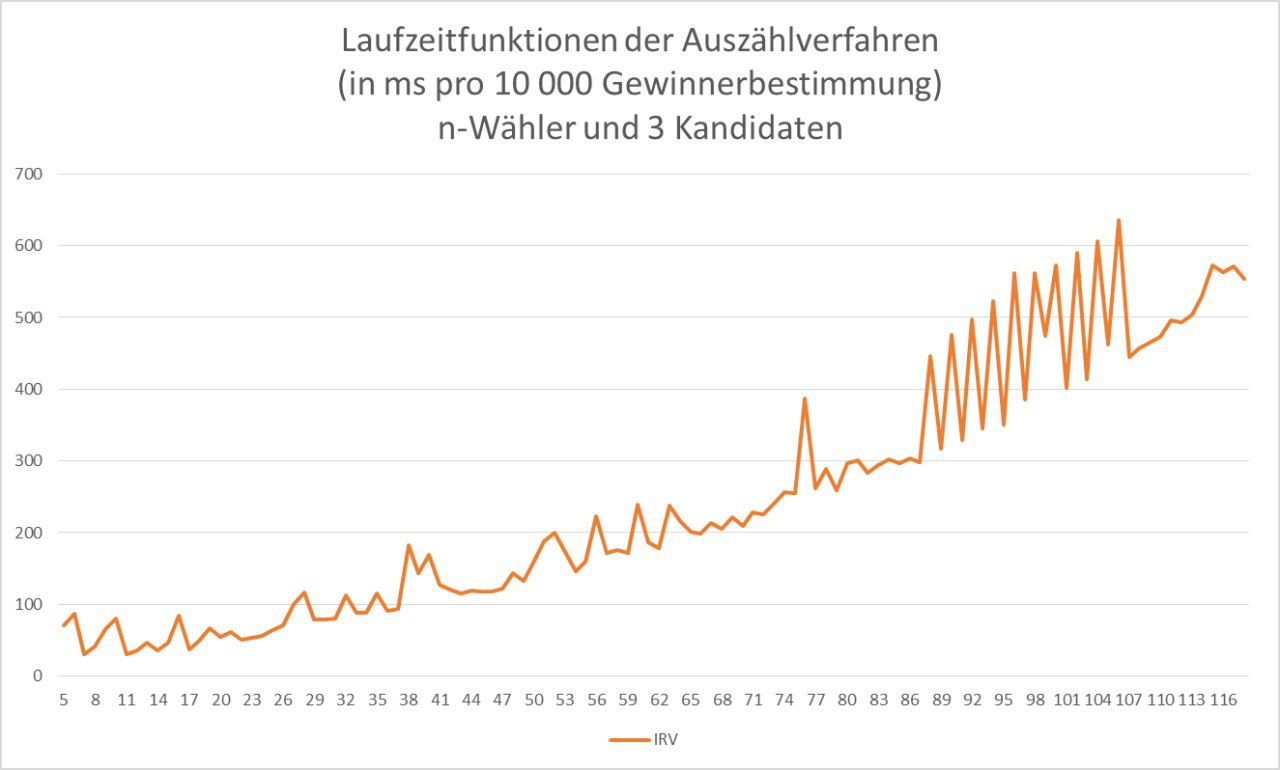
\includegraphics[width=\textwidth]{res/voting_sys_stats/irv_stat.JPG}}
	\caption{\label{fig:irv_stat}
		IRVVotingSystem
	}
\end{figure}

\begin{figure}[ht]
	\fbox{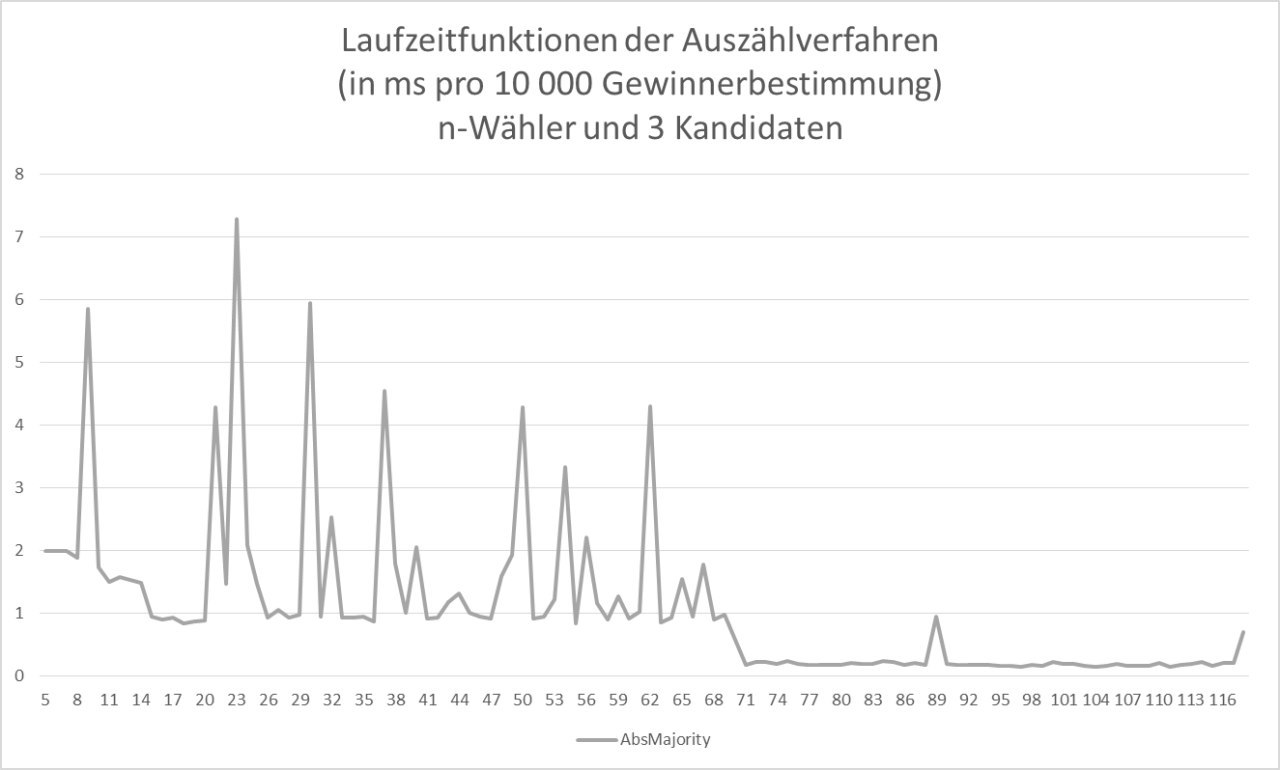
\includegraphics[width=\textwidth]{res/voting_sys_stats/absmaj_stat.JPG}}
	\caption{\label{fig:absmaj_stat}
		AbsoluteMajorityVotingSystem
	}
\end{figure}

\begin{figure}[ht]
	\fbox{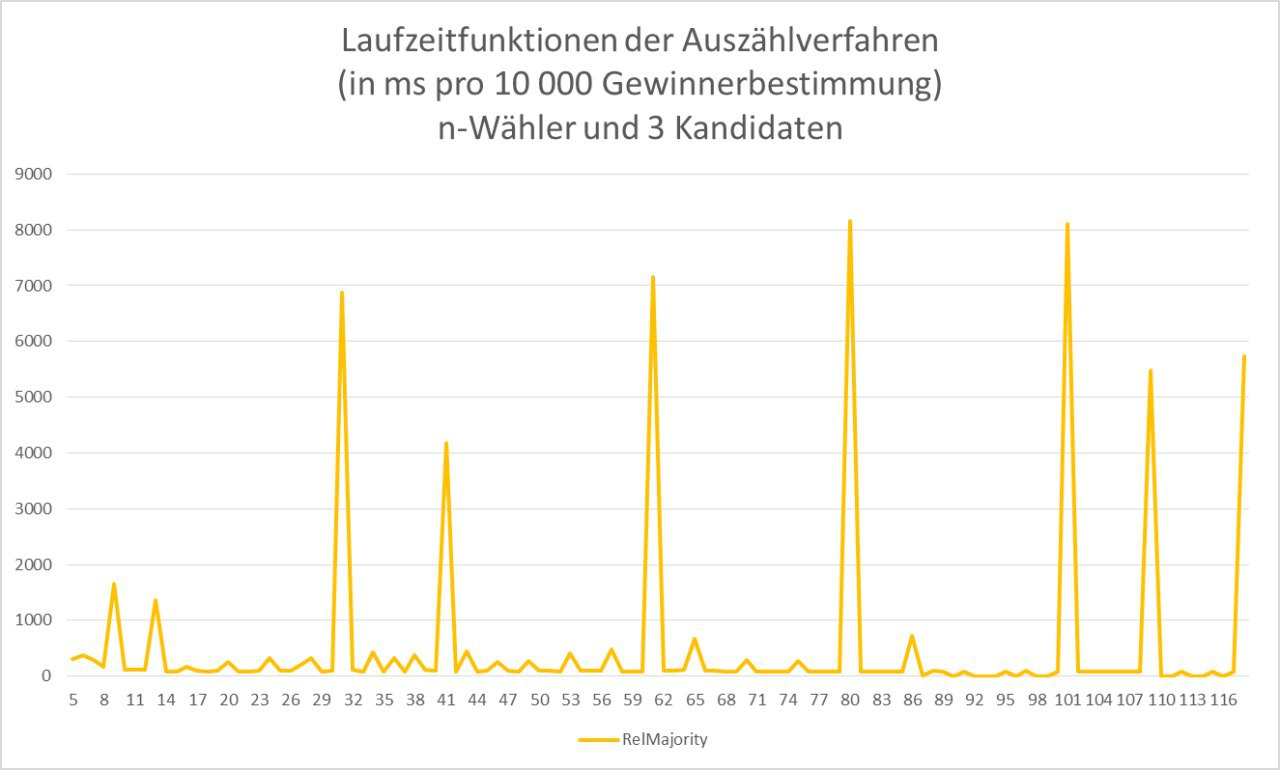
\includegraphics[width=\textwidth]{res/voting_sys_stats/relmaj_stat.JPG}}
	\caption{\label{fig:relmaj_stat}
		RelativeMajorityVotingSystem
	}
\end{figure}

\begin{enumerate}
	\item Schlussfolgerung zur \autoref{fig:irv_stat}: Die Grafik zeigt deutlich, dass mit wachsender Wählerzahl auch die Zeit zur Gewinnermittlung steigt. In diesem Fall ist die Abhängigkeit nicht direkt proportional.
	
	\item Schlussfolgerung zur \autoref{fig:absmaj_stat}: Es keine Zeitabhängigkeit zwichen Wählerzahl und die Zeit zur Gewinnermittlung gibt.
	
	\item Schlussfolgerung zur \autoref{fig:relmaj_stat}: Die Grafik zeigt, dass während der Ausführung des Algorithmus periodisch eine starke Zunahme der Geschwindigkeit auftritt, die erforderlich ist, um den Gewinner zu identifizieren.
\end{enumerate}

\section{GUI-Testplan}
\subsection{Vorgehen}
Der Quellcode der Software besteht zu einem großen Anteil aus Quellcode für die Benutzeroberfläche. Deswegen entschieden wir uns dafür, die Benutzeroberfläche zu testen und einen Plan zu erstellen, der den Testablauf festlegt und dokumentiert. Das automatisierte Testen von Benutzeroberflächen ist schwer und umständlich zu implementieren, deswegen entschieden wir uns für manuelle Benutzeroberflächen-Tests.
\\
Ein Testszenario ist in eine Folge, bestehend aus Testschritten, gegliedert. Ein Testschritt besteht aus einer genauen Beschreibung einer Nutzer-Aktion, welche mit der Benutzeroberfläche interagiert und der erwarteten Reaktion der Benutzeroberfläche. Die testende Person führt in jedem Testschritt die beschriebene Aktion aus und vergleicht die eintretende Reaktion der Benutzeroberfläche mit der erwarteten Reaktion, die im Testschritt beschrieben ist. Gibt es eine Abweichung, so wird dieses Verhalten als Fehler im Issue-Tracker dokumentiert.
\\
Jeder Schritt geht davon aus, dass alle vorherige Schritte erfolgreich ausgeführt wurde. Außerdem wird sich auf die Benutzeroberfläche bezogen die im vorherigen Schritt benutzt wurde, es sei denn es ist anders beschrieben.
\\
Dieser Testplan beinhaltet die im Pflichtenheft beschriebenen Testszenarien. Jedoch wurden diese kombiniert und präziser formuliert.
Das zweite Testszenario wurde nicht in den Testplan integriert, da das benutzte Werkzeug für die Code-Überdeckung Schwierigkeiten hatte das Ergebnis, von mehreren Ausführungen des selben Programmes, zu kombinieren. Nichtsdestotrotz wurde dieses Szenario extern verifiziert und die vorhergesehene Funktionalität sichergestellt.

\subsection{Testplan}
\subsubsection{Voraussetzung}
\begin{enumerate}
		\item Das Blockchain-Netzwerk ist aufgesetzt.
		\item Deutsches locale ist definiert.
\end{enumerate}

\subsubsection{Test}
\teststep{Das Programm ist gestartet.}
		{Das Authentifizierungsmenü des Wahlleiters erscheint}

\begin{figure}[h!]
	\fbox{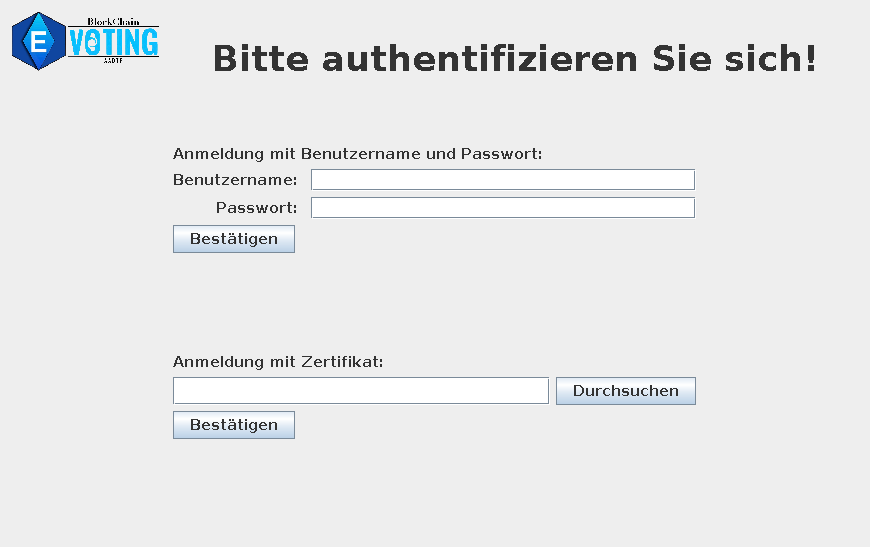
\includegraphics[width=\textwidth]{res/supervisor_authentication.png}}
	\caption{\label{fig:sup_authentication}
		Das Authentifizierungsmenü des Wahlleiters.
	}
\end{figure}

\teststep{}
		{Drücken der oberen \enquote{Bestätigen}-Schaltfläche.}
		{Es erscheint eine Fehlermeldung, die darauf hinweist, dass der Benutzername oder Passwort falsch ist.}

\teststep{Drücken der unteren \enquote{Bestätigen}-Schaltfläche.}
		{Es erscheint eine Fehlermeldung die darauf hinweist, dass das Zertifikat ungültig ist.}

\teststep{\begin{enumerate}
				\item Eingabe des Benutzername des Wahlleiters in das entsprechende Eingabefeld.
				\item Eingabe des Passworts des Wahlleiters in das entsprechende Eingabefeld.
				\item Die obere Schaltfläche \enquote{Bestätigen} drücken.
		\end{enumerate}}
		{Die GUI ändert sich auf die Startseite des Wahlleiters.}

\begin{figure}[h!]
	\fbox{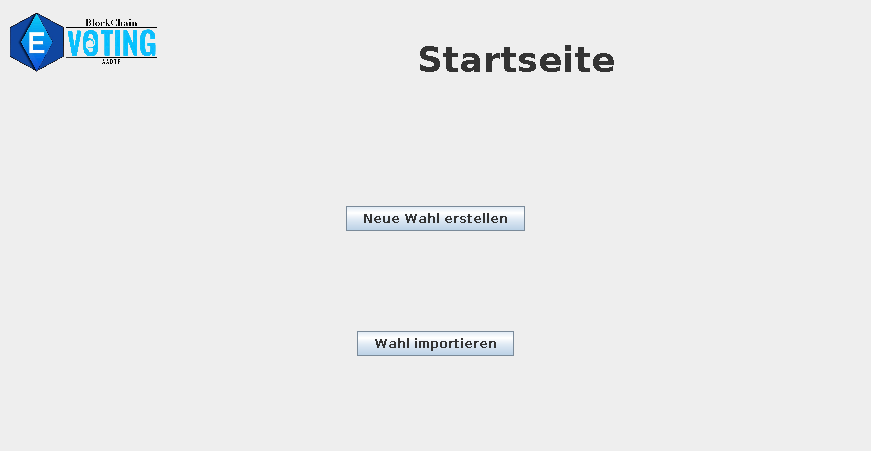
\includegraphics[width=\textwidth]{res/supervisor_frontpage.png}}
	\caption{\label{fig:sup_frontpage}
		Die Startseite des Wahlleiters.
	}
\end{figure}
		
\teststep{Drücken der Schaltfläche \enquote{Neue Wahl erstellen}.}
		{Es erscheint das Konfigurationsmenü.}

\begin{figure}[h!]
	\fbox{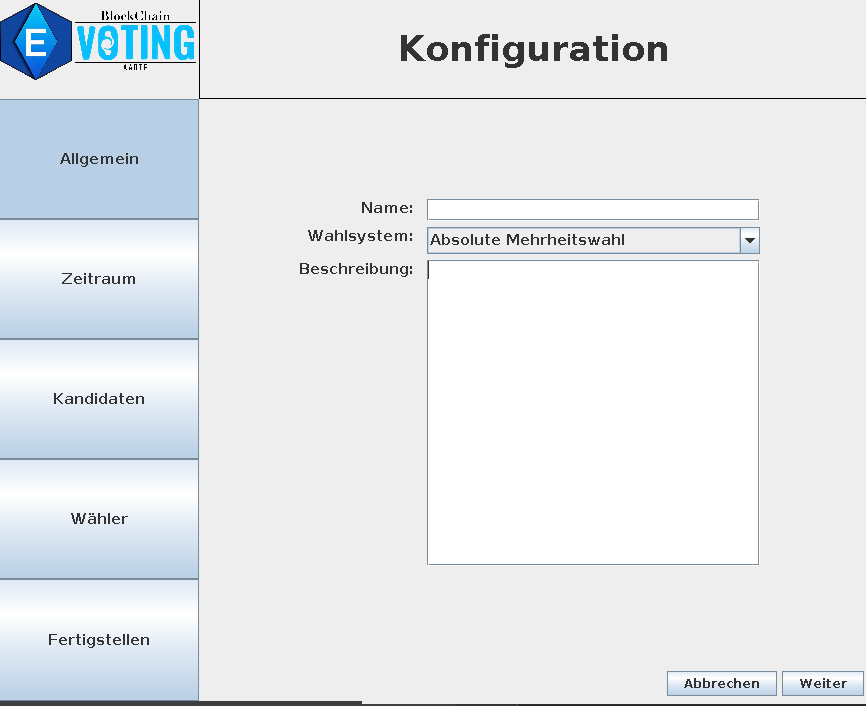
\includegraphics[width=\textwidth]{res/configuration.png}}
	\caption{\label{fig:sup_configuration}
		Das Konfigurationsmenü des Wahlleiters.
	}
\end{figure}

\teststep{Drücken der Schaltfläche \enquote{Fertigstellen}.}
		{Der Fertigstellen-Tab des Konfigurationsmenü wird angezeigt mit folgenden Fehlern:
		\begin{enumerate}
			\item Der Wahlname muss aus mindestem einem Wort bestehen.
			\item Ein End- und Start-Zeitpunkt muss definiert sein.
			\item Es muss mindestens Zwei Kandidaten geben.
			\item Es muss mindestens Zwei Wähler geben.
		\end{enumerate}}

\teststep{\begin{enumerate}
				\item Drücken der Schaltfläche \enquote{Allgemein}.
				\item Eingabe des Namens \enquote{Vorstandswahl 2018} in das Eingabefeld \enquote{Name}.
				\item Auswahl des Wahlsystems \enquote{Relative Mehrheitswahl}.
				\item Eingabe der Beschreibung \enquote{Die Wahl des neuen Vorstands.} in das Eingabefeld \enquote{Beschreibung}.
				\item Drücken der Schaltflache \enquote{Weiter}.
		\end{enumerate}}
		{\begin{enumerate}
				\item Das Konfigurationsmenü wechselt zu dem Zeitraum-Tab.
				\item Der der Name der \enquote{Vorstandswahl 2018} wird als Titel der Wahl angezeigt.
		\end{enumerate}}

\teststep{Drücken der \enquote{Sofort}-Schaltflache.}
		{\begin{enumerate}
				\item Das derzeitige Datum wird in der oberen Datum-Eingabe angezeigt.
				\item Die derzeitige Uhrzeit wird in der oberen Uhrzeit-Eingabe angezeigt.
		\end{enumerate}}
	
\teststep{\begin{enumerate}
				\item Eingabe des aktuellen Datums in die untere Datum-Eingabe.
				\item Eingabe der Aktuellen Uhrzeit plus 5 Minuten in die untere Uhrzeit-Eingabe.
				\item Auswahl der \enquote{Wähler Prozentsatz}-Extrabedingung.
				\item Eingabe 98\% in die Prozent-Eingabe.
				\item Drücken der Schaltfläche \enquote{Weiter}.
		\end{enumerate}}
		{Das Konfigurationsmenü wechselt zu dem Kandidaten-Tab.}

\teststep{Drücke die Schaltfläche \enquote{-}.}
		{Die Liste in dem Konfigurationsmenü ist komplett leer.}
		
\teststep{Drücke die Schaltfläche \enquote{Kandidat Hinzufügen} zweimal.}
		{Zwei Zeilen sind in der Liste erschienen.}
	
\teststep{\begin{enumerate}
			\item Gebe \enquote{Wolfgang Rudolf} in das erste Eingabefeld in der Liste ein.
			\item Gebe \enquote{Sabine Scholl} in das zweite Eingabefeld in der Liste ein.
		\end{enumerate}}
		{}

\teststep{Drücke die Schaltfläche \enquote{Beschreibung}.}
		{Es erscheint ein Beschreibungs-Fenster}
		
\teststep{Gebe die Beschreibung \enquote{Vorstandsvorsitzender seit 10 Jahren.} und drücke die Schaltfläche \enquote{OK}.}
		{Das Beschreiungs-Fenster schließt sich.}
		
\teststep{Drücke die Schaltfläche \enquote{Wähler} im Konfigurationsmenü.}
		{Das Konfigurationsmenü wechselt zum dem Wähler-Tab}

\teststep{\begin{enumerate}
				\item Drücke die Schaltfläche \enquote{Wähler hinzufügen} dreimal.
				\item Gebe den Namen \enquote{Max Mustermann} in das erste Eingabefeld der Liste ein.
				\item Gebe den Namen \enquote{Anna Meier} in das zweite Eingabefeld der Liste ein.
				\item Gebe den Namen \enquote{Ulrich Müller} in das dritte Eingabefeld der Liste ein.
				\item Gebe den Namen \enquote{Erich Schmitt} in das vierte Eingabefeld der Liste ein.
				\item Drücke die Schaltfläche \enquote{-} in der dritten Zeile der Liste.
		\end{enumerate}}
		{Die dritte Zeile verschwindet und die vorherige vierte Zeile wird zur neuen dritten Zeile.}

\teststep{Drücke die Schaltfläche \enquote{Weiter}.}
		{\begin{enumerate}
				\item Es kommt eine Meldung, dass die Wahlkonfiguration erfolgreich akzeptiert wurde.
				\item Es wird der Fertigstellen-Tab in dem Konfigurationsmenü angezeigt.
		\end{enumerate}}

\begin{figure}[h!]
	\fbox{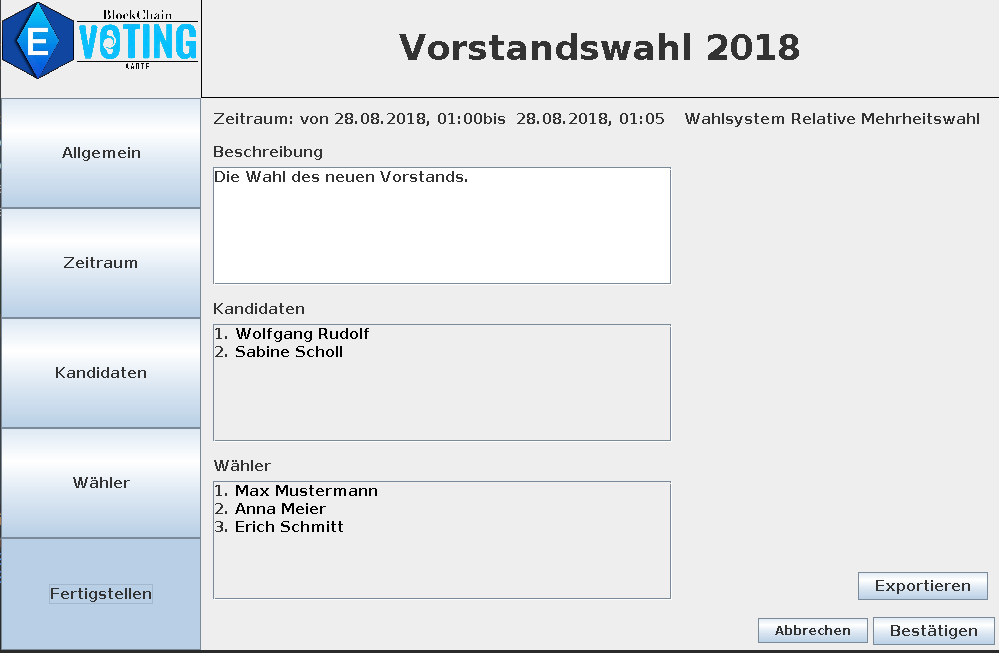
\includegraphics[width=\textwidth]{res/configuration_complete.png}}
	\caption{\label{fig:sup_configuration_complete}
		Der Fertigstellen-Tab des Konfigurationsmenü des Wahlleiters.
	}
\end{figure}


\teststep{Drücke die Schaltfläche \enquote{Exportieren}.}
		{Es erscheint ein Dateiauswahlmenü}

\teststep{Wähle einen Speicherplatz für die zu exportierende Wahl und drücke \enquote{OK}.}
		{Eine Datei ist an diesem Speicherplatz erschienen.}

\teststep{Drücke die \enquote{Abbrechen} Schaltfläche}
		{Das Konfigurationsmenü beendet sich.}

\teststep{Drücke die \enquote{Wahl importieren} Schaltfläche.}
		{Es erscheint ein Dateiauswahlmenü}

\teststep{Wähle die Datei aus die an dem vorher gewählten Speicherplatz erschienen ist und drücke die Schaltfläche \enquote{Öffnen}.}
		{Es erscheint eine Meldung, dass die Konfiguration akzeptiert wurde. Außerdem erscheint ein Konfigurationsmenü, in dem alle vorher eingetragen Daten enthalten sind.}

\teststep{Drücke die \enquote{Bestätigen} Schaltfläche.}
		{\begin{enumerate}
				\item Eine Meldung teilt mit, dass die Wahl erfolgreich gestartet wurde.
				\item Es wird der aktuelle Wahlzustand in der GUI angezeigt.
				\item Links ist eine Tabelle in der jeder Kandidat eine Zeile hat, in welcher der Name und Anzahl Stimmen angezeigt werden. Jede Zeile hat eine eigene Färbung.
				\item In dem Ordner-Verzeichnis, wo das Programm ausgeführt wurde, befindet sich ein Zertifikat für jeden Wähler und ein Zertifikat für den Wahlleiter.
		\end{enumerate}}
	
\begin{figure}[h!]
	\fbox{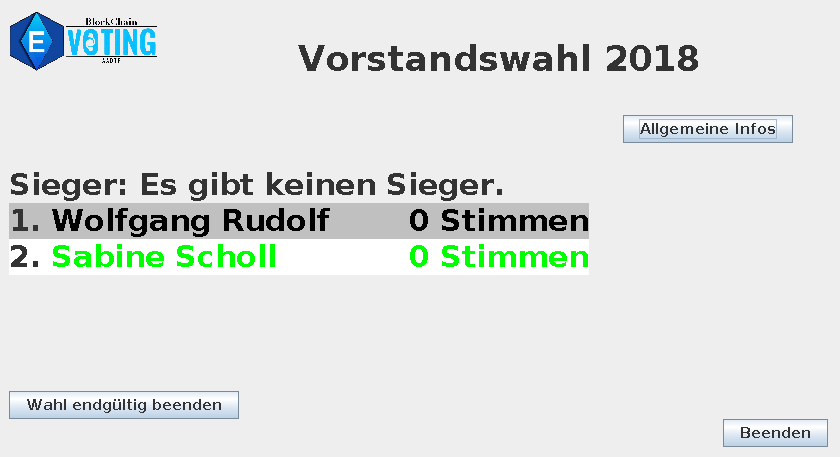
\includegraphics[width=\textwidth]{res/supervisor_result.png}}
	\caption{\label{fig:sup_result}
		Die Ansicht des Wahlleiters während der Wahl.
	}
\end{figure}


\teststep{Drücke die Schaltfläche \enquote{Allgemeine Infos}.}
		{Unter der Schaltfläche erscheint ein Kasten, in dem die Informationen welche konfiguriert wurden angezeigt werden.}

\teststep{Starten des Wähler-Clienten.}
		{Die GUI des Wähler-Clienten wird angezeigt und der Benutzer dazu aufgefordert sein Zertifikat anzugeben.}

\begin{figure}[h!]
	\fbox{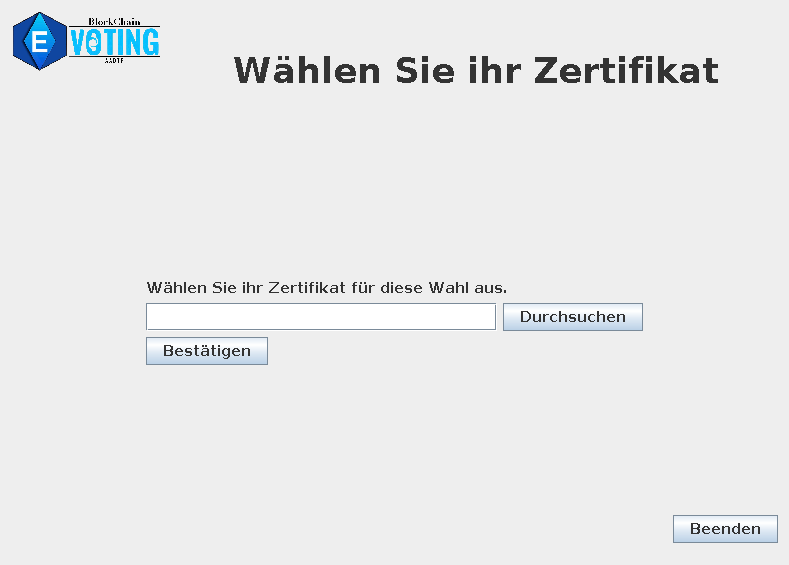
\includegraphics[width=\textwidth]{res/voter_authentication.png}}
	\caption{\label{fig:vot_authentication}
		Das Authentifizierungsmenü des Wählers.
	}
\end{figure}

\teststep{Drücke die Schaltfläche \enquote{Bestätigen}.}
		{Es gibt eine Fehlermeldung, dass der Wähler nicht authentifiziert werden konnte.}

\teststep{Drücken der \enquote{Dursuchen}-Schaltfläche.}
		{Ein Datei-Wahl-Menü erscheint.}
	
\teststep{\begin{enumerate}
				\item Auswählen des Wähler-Zertifikats von "Max Musterman".
				\item \enquote{Öffnen}-Schaltfläche drücken.
		\end{enumerate}}
		{Der Pfad des Zertifikats wird in dem Textfeld neben der "Durchsuchen" Schaltfläche angezeigt.}
		
\teststep{Drücken der \enquote{Bestätigen}-Schaltfläche.}
		{Die GUI ändert sich und zeigt das Wahl-Menü in Form einer Tabelle auf der linken Bildschirmseite, welche einen Zeileneintrag für jeden Kandidaten enthält.}
		
\begin{figure}[h!]
	\fbox{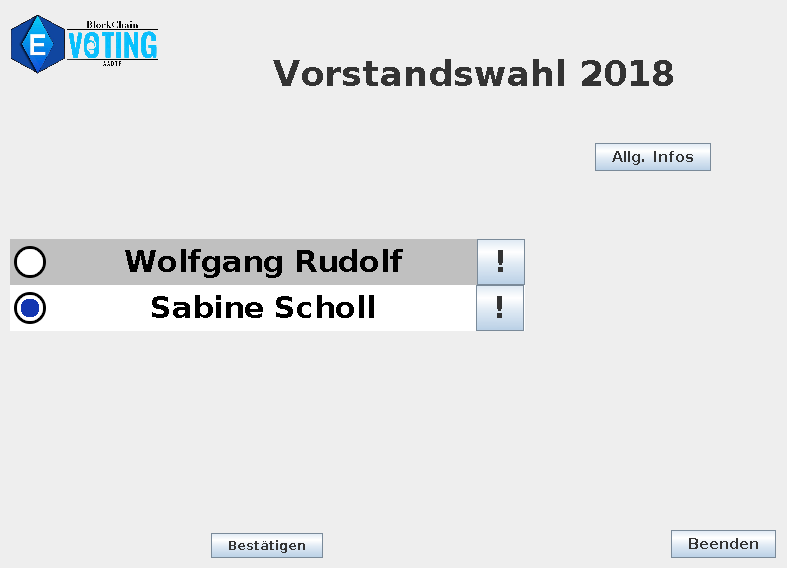
\includegraphics[width=\textwidth]{res/voter_vote.png}}
	\caption{\label{fig:vot_vote}
		Das Wahlmenü des Wählers.
	}
\end{figure}

\teststep{Drücken der \enquote{!}-Schaltfläche in der ersten Zeile der Wahl-Menü-Tabelle.}
		{Es erscheint ein Beschreibungsfenster, in dem die Beschreibung für \enquote{Wolgang Rudolf} steht.}

\teststep{Drücke die Schaltfläche \enquote{Allgemeine Infos}.}
		{Unter der Schaltfläche erscheint ein Kasten, in dem die vorher festgelegten Informationen angezeigt werden.}

\teststep{Klicke den Kreis links von \enquote{Sabine Scholl}.}
		{Der Kreis ist ausgefüllt.}
	
\teststep{Drücke die Schaltfläche \enquote{Bestätigen}.}
		{Es erscheint eine Meldung, die nachfragt, ob man sich seiner sicher Entscheidung sicher sei.}

\teststep{Drücke die Schaltfläche \enquote{Abbrechen} in der Meldung.}
		{Die Meldung verschwindet.}
			
\teststep{Drücke die Schaltfläche \enquote{Bestätigen}.}
		{Es erscheint eine Meldung, die nachfragt, ob man sich seiner sicher Entscheidung sicher sei.}

\teststep{Drücke die Schaltfläche \enquote{OK}.}
		{\begin{enumerate}
			\item Es erscheint eine Meldung, dass die Stimme erfolgreich abgegeben wurde.
			\item Die GUI zeigt nun an, dass man auf das Wahlende warten soll.
			\item Der Ergebnis Bildschirm des Wahlleiters ändert sich und zeigt eine Stimme für \enquote{Sabine Scholl} an.
		\end{enumerate}}
	
\begin{figure}[h!]
	\fbox{
\includegraphics[width=\textwidth]{res/voter_voted.png}}
	\caption{\label{fig:vot_voted}
		Der Wartebildschirm des Wählers.
	}
\end{figure}


\teststep{Warte bis das Ende der Wahl erreicht ist.}
		{\begin{enumerate}
			\item Der Wahlleiter-Klient bekommt eine Meldung das die Wahl zuende ist.
			\item Der Wähler-Klient bekommt eine Meldung das die Wahl zuende ist.
			\item Der Wähler-Klient wechselt auf die Ergebnis Ansicht. Dabei sieht er links für welchen Kandidaten er gewählt hat. Und rechts die Verteilung der Stimmen.
		\end{enumerate}}

\begin{figure}[h!]
	\fbox{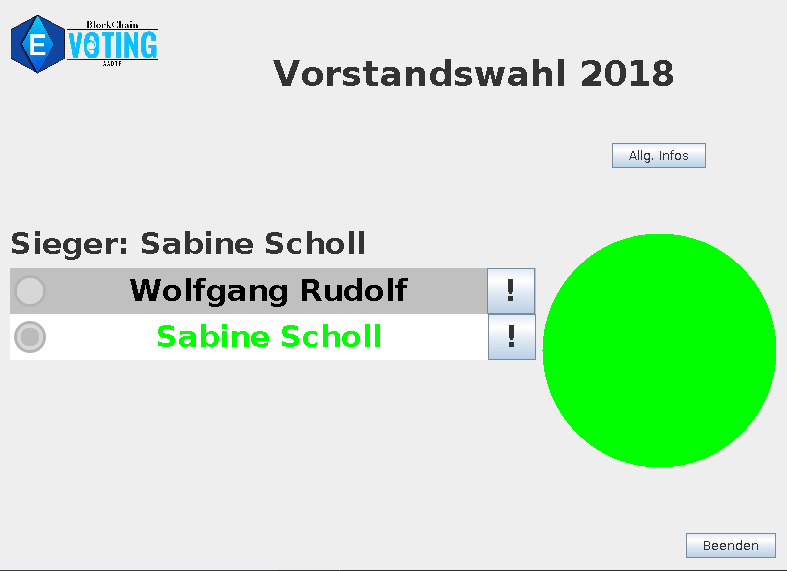
\includegraphics[width=\textwidth]{res/voter_result.png}}
	\caption{\label{fig:vot_result}
		Das Ergebnis des Wählers.
	}
\end{figure}

\teststep{Drücke die Schaltfläche \enquote{Beenden}.}
		{Die GUI des Wählers schließt sich und das Programm terminiert.}


\teststep{Drücke in der Wahlleiter-GUI Schaltfläche \enquote{Wahl endgültig beenden}.}
		{Es erscheint eine Meldung die darauf hinweißt das dieser Schritt nicht rückgangig gemacht werden kann und, dass das Netzwerk neustartet und das Programm terminiert.}

\teststep{Drücke die Schaltfläche \enquote{OK}.}
		{\begin{enumerate}
			\item Der Klient des Wahlleiters terminiert.
			\item Das Netzwerk startet neu. (Es dauert eventuell ein paar Sekunden bis das eintritt.)
		\end{enumerate}}

\section{Code-Überdeckung}
Nach durchführen aller Unit-Tests und dem Manuellen GUI-Testplan erreichen wir eine Linien Code-Überdeckung von 81\%.
Aufgeteilt auf die drei großen Pakete (Model, View und Control) ist die Überdeckung folgendermaßen verteilt:

\begin{table}[h!]
	\begin{tabular}[t]{l r r r}
		Paket & Linien & Methoden & Klassen \\ \hline
		Model & 89\% & 96\% & 100\% \\
		View & 82\% & 82\% & 90\% \\
		Control & 68\% & 87\% & 100\% \\ \hline
		Total & 81\% & 82\% & 88\% \\
	\end{tabular}
\end{table}

Außerhalb von Model, View und Control gab es noch zwei Pakete: Exceptions und Util. Da diese aber Verhältnismäßig eine sehr kleine Linien Anzahl haben, wurden diese weggelassen. Sie sind aber für die Diskrepanz zwischen den Total-Prozenten und Paket-Prozenten der Methoden- und Klassen-Überdeckung verantwortlich.

\section{Gefundene Probleme und deren Lösung}
\subsection{Umkonfigurierung des Netzwerkes}
Wie im Implementierungsbericht erwähnt, wurde, nachdem ein Wähler erfolgreich seine Stimme abgegeben hatte, jedem anderen Wähler ebenfalls der Wartebildschirm des ersten Wählers angezeigt. Dieser Fehler erfolgte durch eine fehlerhafte Konfiguration des Netzwerks. Hierbei wurde für die zur Verfügung gestellten Peers ein falscher Docker-Container von Hyperledger-Fabric gewählt, welcher das registrieren der Peers an der Certificate-Authority nicht korrekt ermöglichte.
\\
Um das übernehmen alter Fehler zu vermeiden wurde das Netzwerk neu aufgesetzt. Die neue Konfiguration verwendet nun die korrekten Docker-Container und ermöglicht die korrekte Kommunikation zwischen Peers und der Certificate-Authority. Das abgeben einer Stimme funktioniert nun für eine beliebige Anzahl an Wählern.

\subsection{Umstrukturierung zu polling-basierter Kommunikation.}
Wie im Entwurfsdokument beschrieben, sollte über die von Hyperledger-Fabric zur Verfügung gestellten Events die Kommunikation mit dem Blockchain-Netzwerk erfolgen, insbesondere um zu erfragen, ob die Wahl beendet ist. Da ausgelöste Events jedoch nicht vom Hyperledger-Fabric-SDK empfangen werden, ist eine solche Implementierung nicht möglich. Daher wurde beschlossen, ein polling-Verfahren zu verwenden. Dabei fragt ein Klient in regelmäßigen Zeitabständen das Blockchain-Netzwerk über Chaincdoe an, ob die Wahl geendet hat.
\\
Die dafür benötigten Änderungen beschränken sich auf das Model-Paket. Bei der Event-basierten Architektur gab es einen Listener, dessen Interface von der SDKConnection definiert und vom Statemanagement implementiert wurde. Diese Listener-Funktionalität wurde komplett entfernt. Das hat zur Folge, dass die Beziehung zwischen der SDKConnection und dem Statemanagement unidirektional ist. Außerdem wurde der Thread, welcher zuvor regelmäßig neue Events in dem Blockchain-Netzwerk ausgelöst hatte, verändert, so dass er in regelmäßigen Zeitabständen ermittelt, ob die Wahl geendet hat.
\\
Insgesamt wurden für diese Änderung 33 Zeilen hinzugefügt und 36 Zeilen gelöscht.

\section{Erfüllte Qualitätsanforderungen}
\paragraph{Korrektheit der Wahlergebnisse}
Der Wähler bekommt erst dann die Benachrichtigung, dass seine Stimme erfolgreich abgegeben wurde, wenn sie auch tatsächlich auf den Ledger geschrieben wurde. Es ist davon auszugehen, dass diese durch die dezentrale Natur des Blockchain Netzwerkes nicht verloren gehen kann.
\paragraph{Protokollierung des Netzwerkes}
Im Ordner /net/logs werden zur Laufzeit des Netzwerkes alle Geschehnisse und Fehler in den entsprechenden Dateien festgehalten.
\paragraph{Unveränderbarkeit der Wahl}
Die Unveränderbarkeit der Wahlkonfiguration ist durch den Chaincode gegeben. Ist einmal ein Block mit der Wahlkonfiguration geschrieben, kann dieser weder verändert noch erneuert werden. Zum erstellen einer neuen Wahl muss der aktuelle Ledger also entfernt werden.
\paragraph{Vermeidung von unlogischen Eigenschaften der Wahl}
Alle im Pflichtenheft angegebenen unlogischen Eigenschaften werden vorm Absenden der Wahl geprüft und im Falle eines Fehlers wird der Nutzer über diesen in Kenntnis gesetzt.
\paragraph{Verhinderung des Double-Spending-Problems}
Wie die Wahlkonfiguration einmalig ist, so ist auch die Stimme des Wählers auf dessen Einzigartige ID gebunden und kann somit kein Zweites mal abgegeben werden.
\paragraph{Vermeidung von ungewollten Enthaltungen}
Sollte ein Wähler keinen Kandidaten ausgewählt haben so ist es ihm auch nicht möglich auf der GUI diese Wahl abzusenden.
\paragraph{Warnungen bei Netzwerkproblemen}
Sollte ein Fehler bei der Kommunikation zum Netzwerk bestehen, so wird dies dem Nutzer kenntlich gemacht, dies geschieht an allen Stellen, bei welchen Kommunikation mit dem Netzwerk stattfindet.


\section{Portabilität}
Die Portabilität der Software wurde getestet unter diversen Linux Distributionen sowie Windows 8.1 und 10.
Die Funktionalität der Software ist auf diesen Plattformen gegeben.
Weiterhin sollte die Funktionalität auch auf Mac OS Plattformen geboten sein, diese konnte aber aufgrund fehlender Ressourcen nicht getestet werden.
\newpage
\section{Performanz}
\paragraph{Vorgehen}
Im Folgenden sollen die Laufzeit und Speicherauslastung von EVote untersucht werden.
Die hierzu erforderlichen Tests wurden auf einem Rechner mit 8 GiB RAM und einem zwei-kernigen \enquote{Intel Core i5-62000U} durchgeführt. Die Daten wurden mithilfe von \textit{YourKit} gesammelt. Laufzeiten wurden auf die effektive Ausführungszeit bereinigt, nur die Zeit in der ein Thread Arbeit verrichtet wurde betrachtet.
\subsection{Testszenario: Erstellen einer Wahl, Export, Starten der Wahl und endgültiges Beenden}
\textbf{Effektive Gesamtlaufzeit:} 7419 ms\\
\textbf{Gesamter Speicherverbrauch:} 113 MiByte \\
\textbf{Speicherverbrauch:}

\begin{table}[h!]
	\begin{tabular}[t]{l r r}
		Paket & Anteil & Größe \\ \hline
		org.hyperledger.* & 39\% & 44.170.288 Byte \\
		javax.imageio.ImageIO & 16\% & 15.789.784 Byte \\
		andere (nicht zuordenbar) & 45\% & 53.039.928 Byte \\
	\end{tabular}
\end{table}
\textbf{Längste Methoden nach Ausführungszeit (mit Untermethoden):}

\begin{table}[h!]
	\begin{tabular}[t]{lrr}
		Methode & Anteil & Zeit \\ \hline
		SupervisorSDKInterfaceImpl.createInstance() & 54\% & 4040 ms \\
		SupervisorSDKInterfaceImpl.registerUser() & 14\% & 1026 ms \\
		Andere (alle < 200 ms) & 32\% & 2353 ms
	\end{tabular}
\end{table}
\subsection{Testszenario: Anmelden, Stimmabgabe bei einer laufenden Wahl}
\textbf{Effektive Gesamtlaufzeit:} 4987 ms\\
\textbf{Gesamter Speicherverbrauch:} 91 MiByte \\
\textbf{Speicherverbrauch:}

\begin{table}[h!]
	\begin{tabular}[t]{l r r}
		Paket & Anteil & Größe \\ \hline
		org.hyperledger.* & 60\% & 54.621.125 Byte \\
		javax.imageio.ImageIO & 8\% & 7.281.324 Byte \\
		andere (nicht zuordenbar) & 32\% & 29.119.928 Byte \\
	\end{tabular}
\end{table}

\textbf{Längste Methoden nach Ausführungszeit (mit Untermethoden):}
\begin{table}[h!]
	\begin{tabular}[t]{lrr}
		Methode & Anteil & Zeit \\ \hline
		org.hyperledger.fabric.sdk.Channel.initialize() & 39\% & 1848 ms \\
		java.io.ObjectInputStream.readObject() & 19\% & 886 ms \\
		SDKInterfaceImpl.createHFClient() & 12\% & 558 ms \\
		Andere (alle < 400 ms) & 30\% & 1695 ms 
	\end{tabular}
\end{table}

\paragraph{Schlussfolgerung}
Die Gesamtlaufzeit wird durch die Kommunikation mit dem Netzwerk, beziehungsweise durch das Hyperledger-SDK dominiert, Optimierungen an EVote-Komponenten sind aufgrund der kurzen Laufzeit derselbigen schwierig und würden im Gesamtbild nur eine minimale Veränderung hervorrufen. Ähnliches gilt für den Speicherbedarf; mit 113 MiByte ist dieser selbst für einen Kleinrechner angemessen.


\end{document}
